\documentclass[letterpaper]{article}
\usepackage{natbib,alifexi}
\usepackage[utf8]{inputenc}

\title{Estimation en temps réel des retards dans un réseau\\ de bus à l'aide de données historiques}
\author{Nikita Marchant$^{1}$\\
\mbox{}\\
$^1$Université Libre de Bruxelles, Département d'Informatique\\
nimarcha@ulb.ac.be}


\begin{document}
\maketitle

\begin{abstract}

\end{abstract}

\section{Introduction}

Power law distributions in Nature usually signal the absence of a
scale in the region where the scaling is observed, and sometimes point
to critical dynamics. In Self-Organized-Criticality (SOC)
\citep{BTW87,BTW88}, for example, power law distributions reveal the
dynamics of an unstable critical point, brought about by slow driving
and a feed-back mechanism between order parameter and critical
parameter.  The critical dynamics is usually described within the
language of second-order phase transitions in condensed matter systems
\citep{SJD}, but it can be shown that SOC-type behavior also occurs
within a dual description in terms of the Landau-Ginzburg equation as
{\em first-order} transitions \citep{GS}.  Indeed, it was shown that a
power law distribution of {\em epoch-lengths}, that is, the time a
particular species dominates the dynamics of an adapting population,
is explained by a self-organized critical scenario \citep{CA2} that
carries the hallmark of first-order phase transitions. Here, we
measure the distribution of abundances of {\em species} and genotypes
in an artificial chemistry, \citep[the Avida Artificial Life
system][]{AB1,OBA} and show that the distribution is scale-free under
a broad class of circumstances, confirming the results reported in
\citep{CA2}.  In the next section, we discuss the first-order dynamics
in more detail and examine ``avalanches of invention'' from the point
of view of a thermodynamics of information. In Section III, we measure
the critical exponent of the power law of genotype abundances in the
limit of infinitesimal driving, i.e., infinitesimal mutation rate, and
discuss the role of the fitness landscape in shaping the
distribution. In Section IV, we repeat the analysis for a higher
taxonomic level (that of species) and discuss its relation to the
geometric distributions found by \citet{BUR90,BUR93}.
Conclusions about the evolutionary process drawn from the data
obtained in this paper are presented in Section V.

\section{Self-Organization in Evolution}

The idea that the evolutionary process occurs in spurts, jumps, and
bursts rather than gradual, slow and continuous changes has been
around for over 75 years \citep{WIL}, but has gained prominence as
``punctuated equilibrium'' through the work of \citet{GE77,GE93}. The
general idea is that evolutionary innovations are not bestowed upon an
existing species as a whole, gradually, but rather by the emergence of
{\em one} better adapted mutant which, by its superiority, serves as
the seed of a new breed that sweeps through an ecological niche and
supplants the species previously occupying it. The global dynamics
thus has a microscopic origin, as shown experimentally, e.g., in
populations of {\it E. Coli} \citep{ECL96}.

Such avalanches can be viewed in two apparently contradictory ways. On
the one hand we may consider the wave of extinction touching all
species that are connected by their ecological relations, a process
akin to percolation and therefore suitably described by the language
of second-order critical phenomena \citep{BS}. Such a scenario relies
on the {\em coevolution} of species (to build their ecological
relations) and successfully describes power-law distributions obtained
from the fossil record \citep{SB96,BP96}. There is, on the other hand,
a description in terms of {\em informational} avalanches that does not
require coevolution and leads to the same statistics, as we show
here. Rather than contradicting the aforementioned picture
\citep{NFST}, we believe it to be complementary.

In the following, we set up a scenario in which {\em information} is
viewed as the agent of self-organization in evolving and adapting
populations. Information is, in the strict sense of Shannon theory, a
measure of correlation between two ensembles: here a population of
genomes and the environment it is adapting to. As described elsewhere
\citep{IAL}, this correlation grows as the population stores more and
more information about the environment via random measurements,
implementing a very effective {\em natural Maxwell demon}. Any time a
stochastic event increases the information stored in the population, a
wave of extinction removes the less adapted genomes and establishes a
new era. Yet, information cannot leave the population as a whole,
which therefore may be thought of as protected by a {\em
semi-permeable membrane} for information, the hallmark of the Maxwell
demon. Let us consider this dynamics in more detail.

The simple living systems we consider here are populations of
self-replicating strings of instructions, coded in an alphabet of
dimension ${\cal D}$ with variable string length $\ell$. The total
number of possible strings is exponentially large. Here, we consider
the subset of all strings currently in existence in a finite
population of size $N$, harboring $N_g$ different types, where
$N_g\ll{\cal D}^\ell$. Each {\em genotype} (particular sequence of
instructions) is characterized by its replication rate $\epsilon_i$,
which depends on the sequence only, while its survival rate is given
by $\epsilon_i/\langle \epsilon\rangle$, in a ``stirred-reactor''
environment that allows a mean-field picture. This average replication
rate $\langle \epsilon\rangle$ characterizes the fitness of the
population as a whole, and is given by
\begin{eqnarray}
\langle \epsilon\rangle=\sum_i^{N_g}\frac{n_i}N \epsilon_i\;,
\end{eqnarray}
where $n_i$ is the {\em occupation number}, or frequency, of genotype
$i$ in the population. As $N_g$ is not fixed in time, the average
depends on time also, and is to be taken over all genotypes currently
living. The total abundance, or size, of a genotype is then
\begin{eqnarray}
s_i=\int_0^\infty n_i(t)\, dt=\int_{T_c}^{T_e}n_i(t)\, dt\;,
\label{size}
\end{eqnarray}
where $T_c$ is the time of creation of this particular genotype, and
$T_e$ the moment of extinction. Before we obtain this distribution in
Avida, let us delve further into the statistical description of the
extinction events.

At any point in time, the fate of every string in the population is
determined by the craftiness of the best adapted member of the
population, described by $\epsilon_{\rm best}$. In this simple,
finite, world, which does not permit strings to affect other members
of the population except by replacing them, not being the best reduces
a string to an ephemeral existence. Thus, every string is
characterized by a {\em relative} fitness, or {\em inferiority}
\begin{eqnarray}
E_i=\epsilon_{\rm best}-\epsilon_i
\end{eqnarray}
which plays the role of an {\em energy} variable for strings of
information {IAL}. Naturally, $\langle E\rangle=0$ characterizes the
{\em ground state}, or vacuum, of the population, and strings with
$E_i>0$ can be viewed as occupying {\em excited} states, soon to
``decay'' to the ground state (by being replaced by a string with
vanishing inferiority). Through such processes, the dynamics of the
system tend to minimize the average inferiority of the population, and
the fitness landscape of replication rates thus provides a Lyapunov
function. Consequently, we are allowed to proceed with our statistical
analysis. Imagine a population in equilibrium, at minimal average
inferiority as allowed by the ``temperature'': the rate (or more
precisely, the probability) of mutation. Imagine further that a
mutation event produces a new genotype, fitter than the others,
exploiting the environment in novel ways, replicating faster than all
the others. It is thus endowed with a new best replication rate,
$\epsilon_{\rm best}^{\rm new}$, larger than the old ``best'' by an
amount $\Delta \epsilon$, and redefining what it means to be
inferior. Indeed, all inferiorities must now be {\em renormalized}:
what passed as a ground state ($E=0$) string before now suddenly finds
itself in an excited state. The seed of a new generation has been
sown, a phase transition must occur. In the picture just described,
this is a first-order phase transition with latent heat
$\Delta\epsilon$ (see Fig.\ref{fig1}), starting at the ``nucleation''
point, and leading to an expanding {\em bubble} of ``new phase''.


\begin{figure}[t]
\begin{center}
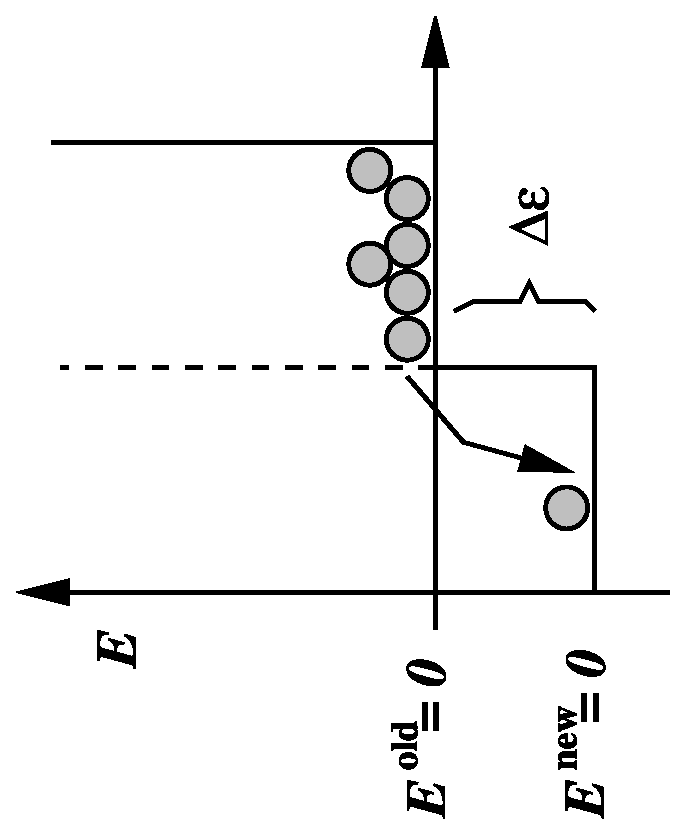
\includegraphics[width=2.1in,angle=-90]{fig1.eps}
\caption{``Energies'' (inferiorities) of strings in a first-order
  phase transition with latent heat $\Delta\epsilon$.}
\label{fig1}
\end{center}
\end{figure}

This bubble expands with a speed given by the Fisher velocity
\begin{eqnarray}
v\sim\sqrt{D\Delta\epsilon}\;, \label{eq4}
\end{eqnarray}
where $D$ is the diffusion coefficient (of information) in this
medium, until the entire population has been converted \citep{CHU}.
This marks the end of the phase transition, as the population returns
to equilibrium via mutations acting on the new species, creating new
diversity and restoring the {\em entropy} of the population to its
previous value. This prepares the stage for a new avalanche, as only
an equilibrated population is vulnerable to even the smallest
perturbation. The system has returned to a critical point, driven by
mutations, self-organized by information.

Thus we see how a first-order scenario, without coevolution, can lead
to self-organized and critical dynamics. It takes place within a
single, finite, ecological niche, and thus does not contradict the
dynamics taking place for populations that span many niches. Rather,
we must conclude that the descriptions complement each other, from the
single-niche level to the ecological web. Let us now take a closer
look at the statistics of avalanches in this model, i.e., at the
distribution of genotype sizes.


\footnotesize
\bibliographystyle{apalike}
\bibliography{example}


\end{document}
